\clearpage
\VerdierPhysicalPageAnchor{0133}%
\begingroup
\small
\setlength{\emergencystretch}{1.5em}%
\setlength{\abovedisplayskip}{1pt plus 1pt minus 1pt}%
\setlength{\belowdisplayskip}{1pt plus 1pt minus 1pt}%
\newcommand{\VerdierHatchTriangle}[3]{%
  \begin{scope}
    \clip (#1) -- (#2) -- (#3) -- cycle;
    \draw[step=.20cm,black!78,line width=.16pt] (-2,-2) grid (7,2);
  \end{scope}}

\VerdierSemanticAnchor{ch2-2-1-13}
\noindent\textbf{2.1.13.}\quad
\VerdierSemanticAnchor{ch2-2-1-13-saturation-direction}%
\emph{If the category $\mathcal D'$ is saturated, the set
$S(\mathcal D')$ is saturated.}
\VerdierSemanticAnchor{ch2-2-1-13-composable-setup}%
Let $f,g,h$ be three composable morphisms such that $fg$ and $gh$ are
elements of $S(\mathcal D')$.

\VerdierSemanticAnchor{ch2-2-1-13-triv-construction}
Using axiom TRIV, one can construct a diagram:

\VerdierSemanticAnchor{ch2-2-1-13-triv-diagram}
\begin{center}
  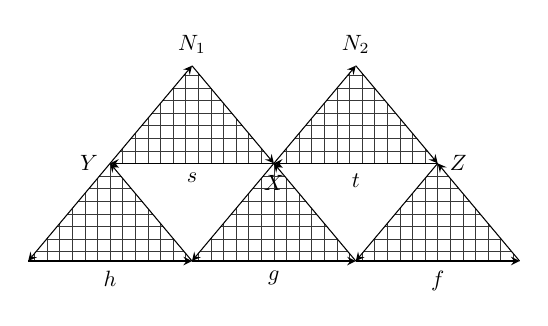
\begin{tikzpicture}[>=stealth,line width=.38pt,scale=.80,transform shape]
    \coordinate (Y)  at (0,0);
    \coordinate (X)  at (2.6,0);
    \coordinate (Z)  at (5.2,0);
    \coordinate (N1) at (1.3,1.55);
    \coordinate (N2) at (3.9,1.55);
    \coordinate (A)  at (-1.3,-1.55);
    \coordinate (Q1) at (1.3,-1.55);
    \coordinate (Q2) at (3.9,-1.55);
    \coordinate (B)  at (6.5,-1.55);

    \VerdierHatchTriangle{Y}{N1}{X}
    \VerdierHatchTriangle{X}{N2}{Z}
    \VerdierHatchTriangle{Y}{A}{Q1}
    \VerdierHatchTriangle{X}{Q1}{Q2}
    \VerdierHatchTriangle{Z}{Q2}{B}

    \draw[->] (Y) -- (N1);
    \draw[->] (N1) -- (X);
    \draw[->] (X) -- node[below=1pt] {$s$} (Y);
    \draw[->] (X) -- (N2);
    \draw[->] (N2) -- (Z);
    \draw[->] (Z) -- node[below=1pt] {$t$} (X);

    \draw[->] (Y) -- (A);
    \draw[->] (A) -- node[below=1pt] {$h$} (Q1);
    \draw[->] (Q1) -- (Y);
    \draw[->] (X) -- (Q1);
    \draw[->] (Q1) -- node[below=1pt] {$g$} (Q2);
    \draw[->] (Q2) -- (X);
    \draw[->] (Z) -- (Q2);
    \draw[->] (Q2) -- node[below=1pt] {$f$} (B);
    \draw[->] (B) -- (Z);

    \node[left=2pt]  at (Y)  {$Y$};
    \node[below=2pt] at (X)  {$X$};
    \node[right=2pt] at (Z)  {$Z$};
    \node[above=2pt] at (N1) {$N_1$};
    \node[above=2pt] at (N2) {$N_2$};
  \end{tikzpicture}
  \quad ,
\end{center}

\VerdierSemanticAnchor{ch2-2-1-13-diagram-interpretation}
\noindent where $N_1$ and $N_2$ are objects of $\mathcal D'$, the five
hatched triangles are distinguished triangles, and the two unhatched
triangles are commutative.

\VerdierSemanticAnchor{ch2-2-1-13-shifted-zero}
It follows that $s[1]t=0$ (1.2.2).
\VerdierSemanticAnchor{ch2-2-1-13-shifted-membership}%
Moreover, by SM1) and SM5), the morphism
$s[1]t$ is an element of $S(\mathcal D')$.

\VerdierSemanticAnchor{ch2-2-1-13-split-triangle}
Hence there exists a distinguished triangle of the form $(Z,Y[2],N,0,u,v)$,
where $N$ is an object of $\mathcal D'$.
\VerdierSemanticAnchor{ch2-2-1-13-direct-summand}%
It follows, using (1.2.6) and TRII, that $Y$ is a direct summand of an object
of $\mathcal D'$.
\VerdierSemanticAnchor{ch2-2-1-13-y-in-dprime}%
Therefore $Y$ is
isomorphic to an object of $\mathcal D'$.

\VerdierSemanticAnchor{ch2-2-1-13-s-triangle}
Using (1.2.4), the fact that $\mathcal D'$ is a triangulated subcategory of
$\mathcal D$, and the distinguished triangle

\begin{center}
  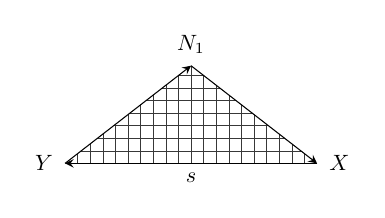
\begin{tikzpicture}[>=stealth,line width=.38pt,scale=.80,transform shape]
    \coordinate (Y)  at (-2,0);
    \coordinate (X)  at (2,0);
    \coordinate (N1) at (0,1.55);
    \VerdierHatchTriangle{Y}{N1}{X}
    \draw[->] (Y) -- (N1);
    \draw[->] (N1) -- (X);
    \draw[->] (X) -- node[below=1pt] {$s$} (Y);
    \node[left=2pt]  at (Y)  {$Y$};
    \node[right=2pt] at (X)  {$X$};
    \node[above=2pt] at (N1) {$N_1$};
  \end{tikzpicture}
\end{center}

\VerdierSemanticAnchor{ch2-2-1-13-g-membership}
\noindent we deduce that $X$ is isomorphic to an object of $\mathcal D'$.
Consequently, the morphism $g$ is an element of $S(\mathcal D')$.

\VerdierSemanticAnchor{ch2-2-1-14}
\medskip
\noindent\textbf{2.1.14.}\quad
\VerdierSemanticAnchor{ch2-2-1-14-saturation-direction}%
\emph{If the set $S(\mathcal D')$ is saturated, the subcategory
$\mathcal D'$ is saturated.}

\VerdierSemanticAnchor{ch2-2-1-14-direct-summand-setup}
Let $X$ be a direct summand of an object of $\mathcal D'$.
\VerdierSemanticAnchor{ch2-2-1-14-first-triangle}%
Using (1.2.6) and
TRII, we see that there exists a distinguished triangle $(X,Y,N,0,u,v)$,
where $N$ is an object of $\mathcal D'$.
\VerdierSemanticAnchor{ch2-2-1-14-zero-morphism}%
Consequently, the zero morphism
$X\to Y$ is a morphism in $S(\mathcal D')$.

\VerdierSemanticAnchor{ch2-2-1-14-sm4-application}
Apply property SM4) to the three morphisms $0\to X\to 0\to Y$.
\VerdierSemanticAnchor{ch2-2-1-14-x-zero-membership}%
It follows
that the morphism $X\to 0$ is an element of $S(\mathcal D')$.

\VerdierSemanticAnchor{ch2-2-1-14-second-triangle}
Hence there exists a distinguished triangle $(X,0,N,0,0,i)$, where $N$ is an
object of $\mathcal D'$.
\VerdierSemanticAnchor{ch2-2-1-14-shift-isomorphism}%
Consequently, the morphism
$N\xrightarrow{i}X[1]$ is an isomorphism. It follows that $X$ is isomorphic
to $N[-1]$, which is an object of $\mathcal D'$.

\VerdierSemanticAnchor{ch2-2-1-14-proposition-complete}
This completes the proof of Proposition (2.1.8).

\VerdierSemanticAnchor{ch2-2-1-14-p134-boundary}
\endgroup
